\begin{savequote}[45mm]
\ascii{Any fool can write code that a computer can understand. Good programmers write code that humans can understand.}
\qauthor{\ascii{- Martin Flower}}
\end{savequote}

\chapter{算法骨架} 
\label{ch:skeleton}

\begin{content}

本章接着驱动实现\ascii{xUnit Mars}引擎的关键路径,并试图推敲出一个测试用例在运行时的完整生命周期。此时,泛型实现的\ascii{TestMethod}也变得越发臃肿。尝试从泛型实现的\ascii{TestMethod}之中,抽取了非泛型实现的逻辑,并形成\ascii{TestCase}漂亮的模板方法,构建了用例执行的主干逻辑。此时,泛型实现的\ascii{TestMethod}退居\ascii{TestCase}的幕后默默地工作。

将复杂的泛型实施封装和隐藏,对外提供非泛型的\ascii{TestCase}编程接口,极大地降低了系统的复杂度和编译时依赖,设计也变得越发有趣多了。

\end{content}

\section{前置}

\begin{content}

一般地,在执行测试前需要预置\ascii{setUp},执行测试环境的初始化工作,完成测试资源的准备。

\subsection{曾经沧海}

重构既有的测试用例使其失败,沿用既有的测试思路,确定\ascii{setUp}事件曾今确实发生过。

\begin{nodiff}{test/mars/core/TestMethodSpec.cc}
\begin{c++}
#include <mars/core/TestMethod.h>
#include <gtest/gtest.h>

namespace {
  bool wasRun = false;
  bool wasSetUp = false;

  struct WasRun {
    void setUp() {
      wasSetUp = true;
    }

    void testMethod() {
      wasRun = true;
    }
  };
}

TEST(WasRunSpec, make_sure_test_method_be_ran) {
  TestMethod<WasRun> test(&WasRun::testMethod);

  ASSERT_FALSE(wasRun);
  test.run();
  ASSERT_TRUE(wasRun);
}

TEST(WasRunSpec, make_sure_setup_was_ran) {
  TestMethod<WasRun> test(&WasRun::testMethod);

  ASSERT_FALSE(wasSetUp);
  test.run();
  ASSERT_TRUE(wasSetUp);
}
\end{c++}
\end{nodiff}

\subsubsection{显式实现}

逻辑较为简单,直接显式实现。此时运行测试,发现测试执行失败。

\begin{diff}{include/mars/core/TestMethod.h}
\begin{minicpp}
template <typename Fixture>
struct TestMethod {
private:
  using Method = void(Fixture::*)();

public:
  TestMethod(Method method)
    : method(method) {}

  void run() {
    (self.*method)();
  }

private:
  Fixture self;
  Method method;
};
\end{minicpp}
\tcblower
\begin{minicpp}
template <typename Fixture>
struct TestMethod {
private:
  using Method = void(Fixture::*)();

public:
  TestMethod(Method method)
    : method(method) {}

  void run() {
    self.setUp();
    (self.*method)();
  }

private:
  Fixture self;
  Method method;
};
\end{minicpp}
\end{diff}

\subsubsection{重置标记}

简单分析,是因为测试之间产生了依赖。引入测试夹具\ascii{WasRunSpec},在\ascii{SetUp}中重置\ascii{wasSetUp, wasRun}标记。

\begin{nodiff}{test/mars/core/TestMethodSpec.cc}
\begin{c++}
#include <mars/core/TestMethod.h>
#include <gtest/gtest.h>

namespace {
  bool wasRun;
  bool wasSetUp;

  struct WasRun {
    void setUp() {
      wasSetUp = true;
    }

    void testMethod() {
      wasRun = true;
    }
  };

  struct WasRunSpec : testing::Test {
  private:
    // IMPORTANT: should reset all flags.
    void SetUp() override {
      wasRun = false;
      wasSetUp = false;
    }
  };
}

TEST_F(WasRunSpec, make_sure_test_method_be_ran) {
  TestMethod<WasRun> test(&WasRun::testMethod);

  ASSERT_FALSE(wasRun);
  test.run();
  ASSERT_TRUE(wasRun);
}

TEST_F(WasRunSpec, make_sure_setup_be_ran) {
  TestMethod<WasRun> test(&WasRun::testMethod);

  ASSERT_FALSE(wasSetUp);
  test.run();
  ASSERT_TRUE(wasSetUp);
}
\end{c++}
\end{nodiff}

测试通过。

\subsubsection{消除重复}

两个测试用例,存在明显的重复设计。重构测试用例,提取公共实现至测试夹具\ascii{WasRunSpec}之中,消除两者之间的重复逻辑。

\begin{nodiff}{test/mars/core/TestMethodSpec.cc}
\begin{c++}
#include <mars/core/TestMethod.h>
#include <gtest/gtest.h>

namespace {
  bool wasRun;
  bool wasSetUp;

  struct WasRun {
    void setUp() {
      wasSetUp = true;
    }

    void testMethod() {
      wasRun = true;
    }
  };

  struct WasRunSpec : testing::Test {
  private:
    void SetUp() override {
      wasRun = false;
      wasSetUp = false;
    }

  protected:
    void makeSure(bool invoked) {
      ASSERT_FALSE(invoked);
      test.run();
      ASSERT_TRUE(invoked);      
    }

  private:
    TestMethod<WasRun> test = &WasRun::testMethod;
  };
}

TEST_F(WasRunSpec, make_sure_test_method_was_ran) {
  makeSure(wasRun);
}

TEST_F(WasRunSpec, make_sure_setup_was_ran) {
  makeSure(wasSetUp);
}
\end{c++}
\end{nodiff}

测试通过,重构完毕。

\subsection{按部就班}

至此,测试用例确定\ascii{setUp}的确发生过,但完全不确定\ascii{setUp}是否在\ascii{testMethod}之前发生。新增一个失败的测试用例,验证\ascii{setUp}在\ascii{testMethod}之前被调用。

做法非常简单,增加一个字符串类型的收集器,当测试逻辑被调用时,追加结果到此收集器。最后断言收集器的顺序是否与预期一致。

\begin{nodiff}{test/mars/core/TestMethodSpec.cc}
\begin{c++}
#include <mars/core/TestMethod.h>
#include <gtest/gtest.h>

namespace {
  bool wasRun;
  bool wasSetUp;
  std::string result;

  struct WasRun {
    void setUp() {
      wasSetUp = true;
      result += "setUp";
    }

    void testMethod() {
      wasRun = true;
      result += "runTest";
    }
  };

  struct WasRunSpec : testing::Test {
  private:
    void SetUp() override {
      wasRun = false;
      wasSetUp = false;
      result.clear();
    }

  protected:
    void makeSure(bool invoked) {
      ASSERT_FALSE(invoked);
      test.run();
      ASSERT_TRUE(invoked);      
    }

  protected:
    TestMethod<WasRun> test = &WasRun::testMethod;
  };
}

TEST_F(WasRunSpec, make_sure_test_method_was_ran) {
  makeSure(wasRun);
}

TEST_F(WasRunSpec, make_sure_setup_was_ran) {
  makeSure(wasSetUp);
}

TEST_F(WasRunSpec, should_setup_before_running_test) {
  test.run();
  ASSERT_EQ("[setUp][runTest]", result);
}
\end{c++}
\end{nodiff}

\subsubsection{消除重复}

使用字符串类型的收集器,其测试更具有覆盖性,它完全覆盖了采用布尔类型\ascii{wasRun, wasSetUp}标记位的方法。为了消除重复的测试逻辑,可以删除标记位\ascii{wasRun, wasSetUp},仅保留收集器\ascii{result}即可。

此时,既有的测试夹具也被一并删除,毕竟此处只有一个测试用例存在。之前,建立测试夹具是为了消除两个测试用例之间的重复实现;现在,删除测试夹具是因为原来的两个测试用例已经被删除,它也没有继续存在的理由。由此可以看出,重构是很自然的过程,应该成为日常的一个习惯。

\begin{nodiff}{test/mars/core/TestMethodSpec.cc}
\begin{c++}
#include <gtest/gtest.h>
#include <mars/core/TestMethod.h>

namespace {
  std::string result;

  struct WasRun {
    void setUp() {
      result += "[setUp]";
    }

    void testMethod() {
      result += "[runTest]";
    }
  };
}

TEST(WasRunSpec, should_setup_before_running_test) {
  TestMethod<WasRun> test(&WasRun::testMethod);
  test.run();
  ASSERT_EQ("[setUp][runTest]", result);
}
\end{c++}
\end{nodiff}

\end{content}

\section{后置}

\begin{content}

\subsection{清仓查库}

测试执行后使用\ascii{tearDown}完成现场清理,释放资源。重构既有的测试用例使其失败,确定\ascii{tearDown}事件发生的顺序与预期相符。

\begin{nodiff}{test/mars/core/TestCaseSpec.cc}
 \begin{c++}
#include <mars/core/TestMethod.h>
#include <gtest/gtest.h>

namespace {
  std::string result;

  struct WasRun {
    void setUp() {
      result += "[setUp]";
    }

    void testMethod() {
      result += "[runTest]";
    }

    void tearDown() {
      result += "[tearDown]";
    }
  };
}

TEST(WasRunSpec, full_life_cycle_for_test_case) {
  TestMethod<WasRun> test(&WasRun::testMethod);
  test.run();
  ASSERT_EQ("[setUp][runTest][tearDown]", result);
}
\end{c++}
\end{nodiff}

\subsubsection{通过测试}

当用例执行完成后,\ascii{TestCase::tearDown}负责清理现场。

\begin{diff}{include/mars/core/TestMethod.h}
 \begin{minicpp}
template <typename Fixture>
struct TestMethod {
private:
  using Method = void(Fixture::*)();

public:
  TestMethod(Method method)
    : method(method) {}

  void run() {
    self.setUp();
    (self.*method)();
  }

private:
  Fixture self;
  Method method;
};
  \end{minicpp}
\tcblower
 \begin{minicpp}
template <typename Fixture>
struct TestMethod {
private:
  using Method = void(Fixture::*)();

public:
  TestMethod(Method method)
    : method(method) {}

  void run() {
    self.setUp();
    (self.*method)();
    self.tearDown();
  }

private:
  Fixture self;
  Method method;
};
  \end{minicpp}
\end{diff}

\subsection{连理分枝}

至此用例运行时的主干逻辑已然形成,即使缺乏异常处理机制。但是,\ascii{TestMethod}携带复杂的模板参数,使用起来极为不便。仔细推敲,\ascii{TestMethod::run}逻辑由三个基本逻辑组成,可以稳定地抽取出来。

\begin{enum}
  \eitem{准备资源: \code{setUp};}
  \eitem{执行测试: \code{runTest};}
  \eitem{释放资源: \code{tearDown}。}
\end{enum}

\subsubsection{提取算法}

\ascii{TestCase::run}是对外公开的唯一入口,它实现了\ascii{xUnit}最核心的高层算法逻辑。用户根据自己的场景定制\ascii{setUp, runTest, tearDown},分别完成资源准备、测试执行和资源清理,实现了高层算法逻辑与底层实现细节的解耦,并且实现了高层算法逻辑的高度复用。

\begin{diff}{include/mars/core/TestCase.h, src/mars/core/TestCase.cc}
 \begin{minicpp}
struct TestCase {
  void run();

  virtual ~TestCase() {}

private:
  virtual void setUp() {}
  virtual void runTest() {}
  virtual void tearDown() {}
};
  \end{minicpp}
\tcblower
 \begin{minicpp}
#include <mars/core/TestCase.h>

void TestCase::run() {
  setUp();
  runTest();
  tearDown();
}
  \end{minicpp}
\end{diff}

需要关注的是,\ascii{TestCase}实现了一个虚拟析构函数。如果不经意地遗忘声明该析构函数为虚拟的\footnote{默认生成的析构函数是公开的、非虚拟的、内联实现的。},则可能招致运行时不确定的行为发生。

\begin{episode}{虚拟析构函数}
\begin{content}

一般地,需要为\emph{多态基类}声明虚拟析构函数;否则,会招致运行时不可预期的行为。一般地,如果一个类包含虚函数时,便将其析构函数声明为虚拟的。

\subsubsection{空实现}

但是,为每个接口类型实现一个空的虚拟析构函数,显得重复而且麻烦。可以引入一个宏定义,自动引入空实现的虚拟析构函数。

 \begin{c++}
namespace details {
  template<typename T>
  struct Trait {
    virtual ~Trait() {}
  };
}

#define TRAIT(trait)  struct trait : ::details::Trait<trait>
#define EXTENDS(...) , ##__VA_ARGS__
 \end{c++}

例如,使用\ascii{TRAIT}宏\footnote{借鉴于\ascii{Scala}语言的关键字\ascii{trait}。使用\ascii{TRAIT}定义接口,一则相比使用宏定义\ascii{INTERFACE},极大地降低名字冲突的可能性;二则\ascii{TRAIT}倡导\ascii{Mixin}组合式的设计方法,有别于传统意义的继承方法。},定义了一个接口类型\ascii{SelfDescribing},它自动拥有虚拟析构函数的默认空实现。

 \begin{c++}
struct Description;

TRAIT(SelfDescribing) {
  virtual void describeTo(Description& desc) const = 0;
};
 \end{c++}

\subsubsection{抽象函数}

此外,定义纯虚函数时,常常会遗忘后面的\ascii{0}。可以引入另外一个宏定义。

 \begin{c++}
#define ABSTRACT(...) virtual __VA_ARGS__ = 0
 \end{c++}

使用\ascii{ABSTRACT}定义,不仅可以抑制不经意地遗漏\ascii{0}的错误,也可以改善\ascii{API}的意图和可读性。

\begin{c++}
struct Description;

TRAIT(SelfDescribing) {
  ABSTRACT(void describeTo(Description& desc) const);
};
\end{c++}

\end{content}
\end{episode}

\subsubsection{扩展方法}

如\refig{simple-test}所示,扩展\ascii{TestCase}只需重写算法子步骤的具体逻辑。例如,\ascii{WasRun}的测试用例,扩展实现\ascii{TestCase}的方法如下代码所示。

\begin{figure}[H]
\centering
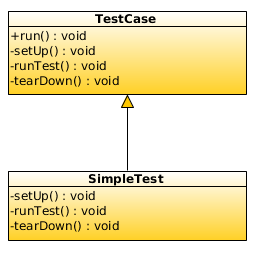
\includegraphics[width=0.4\textwidth]{figures/xunit/simple-test.png}
\caption{模板方法:定义算法骨架}
 \label{fig:simple-test}
\end{figure}

\begin{nodiff}{test/mars/core/TestMethodSpec.cc}
 \begin{c++}
#include "mars/core/TestCase.h"
#include <gtest/gtest.h>

namespace {
  struct WasRun : TestCase {
    bool wasRun = false;

  private:
    void run() override {
      wasRun = true;
    }
  };
}

TEST(WasRunSpec, make_sure_test_method_be_ran) {
  WasRun test;
  test.run();
  ASSERT_TRUE(test.wasRun);
}
  \end{c++}
\end{nodiff}

\begin{episode}{private与override}
\begin{content}

在面向对象程序设计中,需遵循“按接口类型编程”的基本设计原则。在\ascii{C++}设计语言中,基类使用虚函数声明抽象函数,子类使用\ascii{override}覆写虚函数。在编译时,编译器按照基类的接口类型确定函数调用关系。而在运行时,根据对象的具体类型在相应的虚表中检索对应的成员函数,完成运行时多态的调用。

\subsubsection{按接口编程}

从抽象基类的视角看,子类的\ascii{override}函数实现只是它的实现细节而已,应该被声明为\ascii{private}。据此推出一个重要结论:\emph{除非存在特殊需求,都将\ascii{override}函数声明为\ascii{private}}。如此以明确对外声明,在编译时无法通过该具体类型直接调用\ascii{override}函数,而推荐使用抽象的基类型,在运行时完成多态调用。

\subsubsection{例外}

凡事都存在例外,被覆写的析构函数就不应该声明为\ascii{private};否则,无法生成该类型的值对象,否则无法析构该值对象。

\end{content}
\end{episode}

\subsubsection{接口适配}

通过重构,\ascii{TestMethod}成为\ascii{TestCase}的一种实现方法,它基于某个测试方法实现\footnote{测试方法的指针类型为\code{void(Fixture::*)()}。} \ascii{TestCase::run}抽取了用例运行时完整的生命周期,相对较为稳定。

\begin{diff}{include/mars/core/TestMethod.h}
 \begin{minicpp}
template <typename Fixture>
struct TestMethod {
private:
  using Method = void(Fixture::*)();

public:
  TestMethod(Method method)
    : method(method) {}

  void run() {
    self.setUp();
    (self.*method)();
    self.tearDown();
  }

private:
  Fixture self;
  Method method;
};
  \end{minicpp}
\tcblower
 \begin{minicpp}
#include <mars/core/TestCase.h>

template <typename Fixture>
struct TestMethod : TestCase {
private:
  using Method = void(Fixture::*)();

public:
  TestMethod(Method method)
    : method(method) {}

private:
  void setUp() override {
    self.setUp();
  }

  void runTest() override {
    (self.*method)();
  }

  void tearDown() override {
    self.tearDown();
  }

private:
  Fixture self;
  Method method;
};
  \end{minicpp}
\end{diff}

如\refig{testcase-adapter}所示,\ascii{TestMethod}包装了测试方法\code{void(Fixture::*)()}的调用逻辑,且实现了\ascii{TestCase}的具体算法细节。以\ascii{TestMethod}为媒介,任意一个测试方法,都可以适配成为\ascii{TestCase}的一个实例,完美完成\emph{测试方法}到\emph{测试用例}的华丽脱变,这也是\ascii{xUnit Mars}最关键的抽象和设计了。

\begin{figure}[H]
\centering
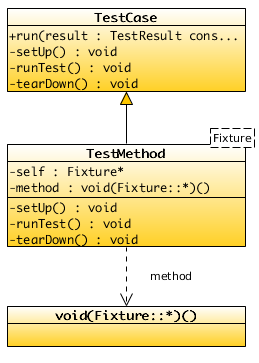
\includegraphics[width=0.4\textwidth]{figures/xunit/testcase-adapter.png}
\caption{适配器与包装器}
 \label{fig:testcase-adapter}
\end{figure}

经过重构,将\ascii{TestMethod}最为稳定的部分已被抽取到\ascii{TestCase}之中,而\ascii{TestCase}是一个普通类,无任何泛型信息,极大地缩小了编译时依赖。\ascii{TestMethod}作为\ascii{TestCase}的实现之一,相对更加稳定和抽象。以后,将不在基于具体的\ascii{TestMethod}讨论问题,而基于抽象的\ascii{TestCase}思考问题。

\end{content}

\section{陷阱}

\begin{content}

存在一个陷阱,存在一个失败的测试用例。因为\ascii{TestMethod}要求\ascii{WasSucc}存在公开的\ascii{setUp, tearDown}成员函数,但\ascii{WasSucc}刚好缺失。

\begin{nodiff}{test/mars/core/WasSuccSpec.cc}
\begin{c++}
#include <mars/core/TestMethod.h>
#include <gtest/gtest.h>

namespace {
  bool wasSucc = false;

  struct WasSucc {
    void testMethod() {
      wasSucc = true;
    }
  };
}

TEST(WasSuccSpec, make_sure_test_method_be_succ) {
  TestMethod<WasSucc> test(&WasSucc::testMethod);
  test.run();
  ASSERT_TRUE(wasSucc);
}
\end{c++}
\end{nodiff}

\subsection{亡羊补牢}

为了修复失败的测试用例,手动给\ascii{WasSucc}添加公开的\ascii{setUp, tearDown}成员函数,且默认实现为空。

\begin{nodiff}{test/mars/core/WasSuccSpec.cc}
\begin{c++}
#include <mars/core/TestMethod.h>
#include <gtest/gtest.h>

namespace {
  bool wasSucc = false;

  struct WasSucc {
    void setUp() {
    }

    void testMethod() {
      wasSucc = true;
    }

    void tearDown() {
    }
  };
}

TEST(WasSuccSpec, make_sure_test_running_be_succ) {
  TestMethod<WasSucc> test(&WasSucc::testMethod);
  test.run();
  ASSERT_TRUE(wasSucc);
}
\end{c++}
\end{nodiff}

显然,默认空实现的\ascii{setUp, tearDown}具有普遍性。每次逼迫用户空实现\ascii{setUp, tearDown},必然造成客户代码的大量重复设计。

\subsection{消除重复}

为了消除重复,提取抽象\ascii{TestFixture},其包含了\ascii{setUp, tearDown}的默认空实现。

\begin{nodiff}{include/mars/core/TestFixture.h}
\begin{c++}
struct TestFixture {
  virtual void setUp() {}
  virtual void tearDown() {}
  
  virtual ~TestFixture() {}
};
\end{c++}
\end{nodiff}

将\ascii{TestFixture}注入给\ascii{WasSucc},消除了\ascii{WasSucc}的空实现。

\begin{diff}{test/mars/core/WasSuccSpec.cc}
\begin{minicpp}
#include <mars/core/TestMethod.h>
#include <gtest/gtest.h>

namespace {
  bool wasSucc = false;

  struct WasSucc {
    void setUp() {
    }

    void testMethod() {
      wasSucc = true;
    }

    void tearDown() {
    }
  };
}

TEST(WasSuccSpec, make_sure_test_running_is_succ) {
  TestMethod<WasSucc> test(&WasSucc::testMethod);
  test.run();
  ASSERT_TRUE(wasSucc);
}
\end{minicpp}
\tcblower
\begin{minicpp}
#include <mars/core/TestMethod.h>
#include <mars/core/TestFixture.h>
#include <gtest/gtest.h>

namespace {
  bool wasSucc = false;

  struct WasSucc : TestFixture {
    void testMethod() {
      wasSucc = true;
    }
  };
}

TEST(WasSuccSpec, make_sure_test_running_is_succ) {
  TestMethod<WasSucc> test(&WasSucc::testMethod);
  test.run();
  ASSERT_TRUE(wasSucc);
}
\end{minicpp}
\end{diff}

同理,测试用例\ascii{WasRun}也可以注入\ascii{TestFixture}。此时,使用\ascii{override}可以增强编译时的安全性。

\begin{diff}{test/mars/core/TestMethodSpec.cc}
\begin{minicpp}
#include <mars/core/TestMethod.h>
#include <gtest/gtest.h>

namespace {
  std::string result;

  struct WasRun {
    void setUp() {
      result += "[setUp]";
    }

    void testMethod() {
      result += "[runTest]";
    }

    void tearDown() {
      result += "[tearDown]";
    }
  };
}

TEST(WasRunSpec, full_life_cycle_for_test_case) {
  TestMethod<WasRun> test(&WasRun::testMethod);
  test.run();
  ASSERT_EQ("[setUp][runTest][tearDown]", result);
}
\end{minicpp}
\tcblower
\begin{minicpp}
#include <mars/core/TestMethod.h>
#include <mars/core/TestFixture.h>
#include <gtest/gtest.h>

namespace {
  std::string result;

  struct WasRun : TestFixture {
    void setUp() override {
      result += "[setUp]";
    }

    void testMethod() {
      result += "[runTest]";
    }

    void tearDown() override {
      result += "[tearDown]";
    }
  };
}

TEST(WasRunSpec, full_life_cycle_for_test_case) {
  TestMethod<WasRun> test(&WasRun::testMethod);
  test.run();
  ASSERT_EQ("[setUp][runTest][tearDown]", result);
}
\end{minicpp}
\end{diff}

\subsection{私有继承}

得益于\ascii{TestFixture}的抽象,\ascii{TestCase}也获得了代码复用的机会,进一步消除重复逻辑。此处使用私有继承,并非公有继承,因为\ascii{setUp, tearDown}只是\ascii{TeseCase::run}的一个具体实现细节。

\begin{diff}{include/mars/core/TestCase.h}
 \begin{minicpp}
struct TestCase {
  void run();

  virtual ~TestCase() {}

private:
  virtual void setUp() {}
  virtual void runTest() {}
  virtual void tearDown() {}
};
  \end{minicpp}
\tcblower
 \begin{minicpp}
#include <mars/core/TestFixture.h>

struct TestCase : private TestFixture {
  void run();

private:
  virtual void runTest() {}
};
  \end{minicpp}
\end{diff}

\subsection{动而若静}

抽象的\ascii{TestFixture},具有运行时多态的特性,可注入到\ascii{TestCase}之中。但是,当被注入到\ascii{WasSucc}之中,被\ascii{TestMethod}按照''鸭子编程''的方式被静态调用。当用户需要重写\ascii{setUp, tearDown}时,用户则不得不\ascii{public}该\ascii{override}实现函数。

仔细推敲,\ascii{TestMethod}中直接基于模板参数\ascii{Fixture}进行编程,违反了''按照接口编程''的设计原则。因此,在\ascii{TestMethod}中增加\code{TestFixture& fixture = self}类内初始化语句,使得调用\ascii{setUp, tearDown}时基于抽象的\ascii{TestFixture}接口类型实现运行时多态。而\code{(self.*method)()}则使用具体的子类型实现编译时多态。动静相辅、协同工作,充分体现了\ascii{C++}无以伦比的设计美感。

\begin{nodiff}{include/mars/core/TestMethod.h}
 \begin{c++}
#include <mars/core/TestCase.h>

template <typename Fixture>
struct TestMethod : TestCase {
private:
  using Method = void(Fixture::*)();

public:
  TestMethod(Method method)
    : method(method) {}

private:
  void setUp() override {
    fixture.setUp();
  }

  void runTest() override {
    (self.*method)();
  }
  void tearDown() override {
    fixture.tearDown();
  }

private:
  Fixture self;
  Method method;
  TestFixture& fixture = self;
};
  \end{c++}
\end{nodiff}

得益于\ascii{TestMethod}动而若静的优秀特性,重写\ascii{WasRun}的\ascii{setUp, tearDown}时,可以将其声明为\ascii{private},不必像之前被强约束必须声明为\ascii{public}。

\begin{nodiff}{test/mars/core/WasRunSpec.h}
 \begin{c++}
#include <mars/core/TestMethod.h>
#include <gtest/gtest.h>

namespace {
  std::string result;

  struct WasRun : TestFixture {
    void testMethod() {
      result += "[runTest]";
    }

  private:
    void setUp() override {
      result += "[setUp]";
    }

    void tearDown() override {
      result += "[tearDown]";
    }
  };
}

TEST(WasRunSpec, full_life_cycle_for_test_case) {
  TestMethod<WasRun> test(&WasRun::testMethod);
  test.run();
  ASSERT_EQ("[setUp][runTest][tearDown]", result);
}
  \end{c++}
\end{nodiff}

\end{content}

\section{策略}

\begin{content}

模板方法模式与策略模式都可以用来分离高层的算法与具体的实现细节。之前已经看到了模板方法的实现,接下来探讨策略模式实现的效果,并从中对比两者之间的差异,从而指导设计的权衡与取舍。

\subsubsection{测试用例}

相对于模板方法,此处需要额外地引入\ascii{TestCaseRunner}。

\begin{diff}{test/mars/core/TestCaseSpec.cc(左:模板方法;右:策略模式)}
 \begin{minicpp}
#include <mars/core/TestCase.h>
#include <gtest/gtest.h>

namespace {
  struct WasRun : TestCase {
    std::string result;

  private:
    void setUp() override {
      result += "setUp";
    }

    void runTest() override {
      result += "runTest";
    }

    void tearDown() override {
      result += "tearDown";
    }
  };
}

TEST(WasRunSpec, full_life_cycle_for_test_case) {
  WasRun test;
  test.run();
  ASSERT_EQ("[setUp][runTest][tearDown]", test.result);
} 
  \end{minicpp}
\tcblower
 \begin{minicpp}
#include <mars/core/TestCase.h>
#include <gtest/gtest.h>

namespace {
  struct WasRun : TestCase {
    std::string result;

  private:
    void setUp() override {
      result += "setUp";
    }

    void runTest() override {
      result += "runTest";
    }

    void tearDown() override {
      result += "tearDown";
    }
  };
}

TEST(WasRunSpec, full_life_cycle_for_test_case) {
  WasRun test;
  TestRunner(test).run();
  ASSERT_EQ("[setUp][runTest][tearDown]", test.result);
}
 \end{minicpp} 
\end{diff}

\subsubsection{通过测试}

两种实现方法差异非常明显。

\begin{enum}
  \eitem{模板方法}
\begin{enum}
  \eitem{使用继承,子类覆写算法子步骤;}
  \eitem{抽象基类\code{TestCase}组织高层算法逻辑,该方法对外公开;}  
  \eitem{抽象基类\code{TestCase}使用\code{private}声明抽象的算法子步骤。}  
\end{enum}
  \eitem{策略模式}
\begin{enum}
  \eitem{使用委托,策略对象覆写算法子步骤;}
  \eitem{额外引入具体类\code{TestCaseRunner},负责组织高层算法逻辑;}  
  \eitem{\code{TestCase}成为\code{TestCaseRunner}的一个抽象策略;}
  \eitem{\code{TestCase}使用\code{public}声明抽象的算法子步骤。}
\end{enum}
\end{enum}

\begin{diff}{include/mars/core/TestCase.h(左:模板方法;右:策略模式)}
 \begin{minicpp}
struct TestCase {
  void run();  
  virtual ~TestCase() {}
  
private:
  virtual void setUp() {}
  virtual void runTest() {}
  virtual void tearDown() {}
};
\end{minicpp}
\tcblower
 \begin{minicpp}
struct TestCase {
  virtual void setUp() {}
  virtual void runTest() {}
  virtual void tearDown() {}

  virtual ~TestCase() {}
}; 

struct TestCaseRunner {
  TestCaseRunner(TestCase& test);
  void run();

private:
  TestCase& test;
};
\end{minicpp} 
\end{diff}

\begin{diff}{src/mars/core/TestCase.cc(左:模板方法;右:策略模式)}
 \begin{minicpp}
#include "mars/core/TestCase.h"

void TestCase::run() {
  setUp();
  runTest();
  tearDown();
};
\end{minicpp}
\tcblower
 \begin{minicpp}
#include "mars/core/TestCase.h"

TestCaseRunner::TestCaseRunner(TestCase& test)
  : test(test) {}

void TestCaseRunner::run() {
  test.setUp();
  test.runTest();
  test.tearDown();
}
\end{minicpp} 
\end{diff}

\subsection{设计权衡}

使用模板方法,\ascii{WasRun}通过继承方式直接复用了\ascii{TestCase::run}高层算法逻辑。但继承是一种强依赖,增强了\ascii{WasRun}与\ascii{TestCase}之间的耦合关系。

\begin{figure}[H]
\centering
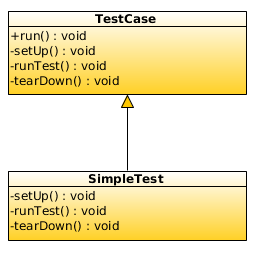
\includegraphics[width=0.4\textwidth]{figures/xunit/simple-test.png}
\caption{模板方法:使用继承}
 \label{fig:simple-test}
\end{figure}

使用策略方法,\ascii{TestCaseRunner}高层算法逻辑与\ascii{WasRun}是解耦的,但额外地引入类\ascii{TestCaseRunner}。

\begin{figure}[H]
\centering
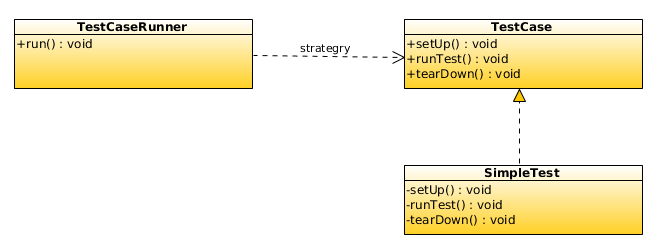
\includegraphics[width=1.0\textwidth]{figures/xunit/simple-test-strategry.png}
\caption{策略对象:使用委托}
 \label{fig:simple-test-strategry}
\end{figure}

既然两个方案都有优缺点,到底应该采用哪个方案呢?如果优选模板方法,其一,使用策略方法,需要建立额外的委托关系,不仅增加了类的数目,而且因“中间人”的委托关系使得设计变得更加复杂。其二,观察\ascii{TestCaseRunner::run}的实现,其实现基本完全委托给了策略对象\ascii{TestCase}。

\begin{nodiff}{src/mars/core/TestCase.cc:中间人}
\begin{c++}
void TestCaseRunner::run() {
  test.setUp();
  test.runTest();
  test.tearDown();
}
\end{c++}
\end{nodiff}

按照迪米特法则,这段高层算法逻辑应该搬迁至策略对象\ascii{TeseCase}。据此实施重构将\ascii{TestCaseRunner::run}搬迁至\ascii{TestCase::run}。此时\ascii{TestCaseRunner}就成为一个空类,根本就没有存在的理由。因此,按照迪米特法则,也应优选模板方法。

如果优选模板方法,因引入继承从而增强了\ascii{TestCase}与\ascii{WasRun}的耦合关系。考虑到\ascii{WasRun}是\ascii{xUnit Mars}最小调度单位,相对稳定,变化不大。也就是说,两者之间的耦合关系仅局部于\ascii{WasRun}内部,不会被传播到其他地方,满足局部化原则,这是完全可以接受的设计。

结论:此时此例,优选\emph{模板方法},而不是\emph{策略}。

\begin{episode}{struct与class}
\begin{content}

关键字\ascii{struct}是\cpp{}继承自\clang{}的一项遗产。作为更加贴切的词汇,\ascii{class}被引入\cpp{},用来表示\emph{类}。但是,\cpp{}增强了\ascii{struct}既有的语义,赋予了\ascii{class}同等的超能力。这样的决策引入了一个选择的难题:如何明确地界定\ascii{struct}与\ascii{class}使用的标准呢? 

这个问题在社区内也并无定论,甚至\cpp{}的发明者\ascii{Bjarne Stroustrup}也无法给出明确的建议。在语法层上,\ascii{struct}和\ascii{class}的差异体现在\emph{默认可见性}:\ascii{struct}默认为\ascii{public},而\ascii{class}则为\ascii{private}。表面上,两者仅存在语法层面的外在差异性,实则存在价值观的潜在差异性。\footnote{本节摘自袁英杰简书:\href{https://www.jianshu.com/p/04974b9a9c68}{https://www.jianshu.com/p/04974b9a9c68}}

\subsubsection{误区}

社区常遵循这样一个规则:使用\ascii{struct}定义数据,不应该定义行为;否则,就使用\ascii{class}定义类。表面看似合理,实则是一个误区。

当然,如果使用\cpp{}开发一个库,并提供一套可供\clang{}语言调用的接口,这个规定是合理的。如果不是基于此类目的,这个规则便是自找麻烦。因为一个类型是否应该定义行为,是随软件演进过程而动态变化的。最初定义的时候,可能以持有数据为主要目的,但无法确保随后不会因为某种目的而为其添加一个方法,简单举例说明。

存在一个结构体\ascii{Rectangle}表示矩形,这是一个纯数据的结构体。

\begin{c++}
struct Rectangle {
  int width;
  int height;
};
\end{c++}

随后,发现客户代码出现大量重复设计。

\begin{c++}
Rectangle r;

r.width = 2;
r.heigth = 4;

bool area = r.width * r.height;
\end{c++}

为了消除重复,可以提取一个初始化函数。

\begin{c++}
void init_rectangle(Rectangle* r, int width, int height) {
  r->width = width;
  r->width = height;
}

int get_area_rectangle(Rectangle* r) {
  return r->width * r->height;
}
\end{c++}

客户如此方式使用这两个\ascii{API}。

\begin{c++}
Rectangle r;
init_rectangle(&r, 2, 4);

int area = get_area_rectangle(&r);
\end{c++}

这是\clang{}语言典型的实现方法。殊途同归,老练的\ascii{C++}程序员,会将其搬迁至成员函数。

\begin{c++}
struct Rectangle {
  Rectangle(int width, int height) : width(width), height(height) {
  }

  int getArea() const {
    return width * height;
  }

  int width;
  int height;
};
\end{c++}

这种做法不仅没有引入任何额外的内存和性能开销。甚至,由于使用了初始化列表,它的性能还略微得到改善。除此之外,还收获了一些其它好处。

\begin{enum}
  \eitem{增强了内聚性:数据与行为在同一个类域内;} 
  \eitem{增强了安全性: 避免对象不经意地发生未初始化的错误;} 
  \eitem{增强了可理解性:客户代码更加的简洁,直观。} 
\end{enum}

而遵循上述规则,则需要将\ascii{Rectangle}修正使用\ascii{class}。但是,这需要在所有的客户代码中,将前置声明\ascii{struct Rectangle}修正为\ascii{class Rectangle};否则,编译期将提示告警信息。显然,这个规则不能支持软件设计的长期演进的需求。

以这种原则来区分使用\ascii{struct},还是\ascii{class},不会带来任何好处,相反只会带来一堆麻烦。于是,不难得出这样的结论:只应该坚持使用其中一个。问题归结于:到底是哪个更好呢?

\subsubsection{接口定义时的差异}

\begin{c++}
class Runnable {
public:
  virtual void run() = 0;
  virtual ~Runnable() {}
};

struct Runnable {
  virtual void run() = 0;
  virtual ~Runnable() {}
};
\end{c++}

两者差别甚微,但却体现了不同的价值观。对于一个纯虚类,从逻辑上本来就是一个只有公开方法声明,没有实现细节的接口类型。在这样的契约关系下,再通过\ascii{public}指明其公开性,纯属画蛇添足。

懒惰的我讨厌冗余,讨厌重复。更何况从平衡和美感的角度看,那个横立的\ascii{public}犹如洁白墙面上的一沫蚊子血,显得格外刺眼。

\subsubsection{继承时的差异}

\begin{c++}
class TestCase : TestFixture, public Test {
  // ...
};

struct TestCase : private TestFixture, Test {
  // ...  
};
\end{c++}

在\ascii{C++}编程实践中,至少$90\%$的情况都会使用公有继承。这就意味着,如果在绝大多数情况下,都要重复地指明\ascii{public},显然不是一个理性的选择。

\subsubsection{类定义的差异}

\begin{c++}
class TestCase : TestFixture, public Test {
  std::string name;

public:
  explicit TestCase(const std::string& name);
};

struct TestCase : private TestFixture, Test {
  explicit TestCase(const std::string& name);

private:
  std::string name;
};
\end{c++}

一般地,常将重要的、用户关心的组件常放于前面,并使用默认的可见性对外公开。使用\ascii{class}常将私有数据放在前面,而将公开接口放在后面。与之相反,使用\ascii{struct}常将公开接口放在前面,而将私有数据放在后面。另外,计算机工业界普遍认为数据结构与算法才是程序设计的核心,理解程序的行为得先从数据结构入手。在这样的价值观驱动下,把私有数据放在前面合乎情理。

随着软件规模的剧增,现代软件工程普遍价值观也发生了巨大变化。尤其\emph{信息隐藏}与\emph{封装}的思想得到工业实践的有效检验。在这种思潮的推动下,封装成为隔离变化的有效工具。通过对客户提供抽象接口,隐藏实现细节;让客户代码只能依赖于更稳定的抽象,与易于变化的实现细节进行隔离,从而让客户代码更加稳定。因此,现代编程语言语言,大多默认将公开接口放在类的前面,而将不稳定的、易变化的私有数据放在后面,甚至利用特殊手段隔离私有数据,尽量使其与客户代码解耦和。

据此推理,\ascii{struct}的特性符合\emph{信息隐藏}与\emph{封装}的基本原则。

\subsubsection{一致性}

需要强调的是,无论\ascii{class}还是\ascii{struct},都应该坚持选择其中一个,而不是混合使用。否则,在大量使用前置声明的情况下,一旦某个使用\ascii{struct}改为\ascii{class},所有前置声明都需要修改。或许编译器并不认为这种不一致是一种错误,但那些不断骚扰的警告亦不胜其烦。

\end{content}
\end{episode}

\end{content}
